\section{Energiespeicher}

Die gesamte Energiespeicherung wird in einzelne Komponenten aufgeteilt, wobei Abbildung \ref{fig:blockschaltbild} einen groben Überblick über den Aufbau gibt.

\begin{figure}[H]
	\begin{center}
		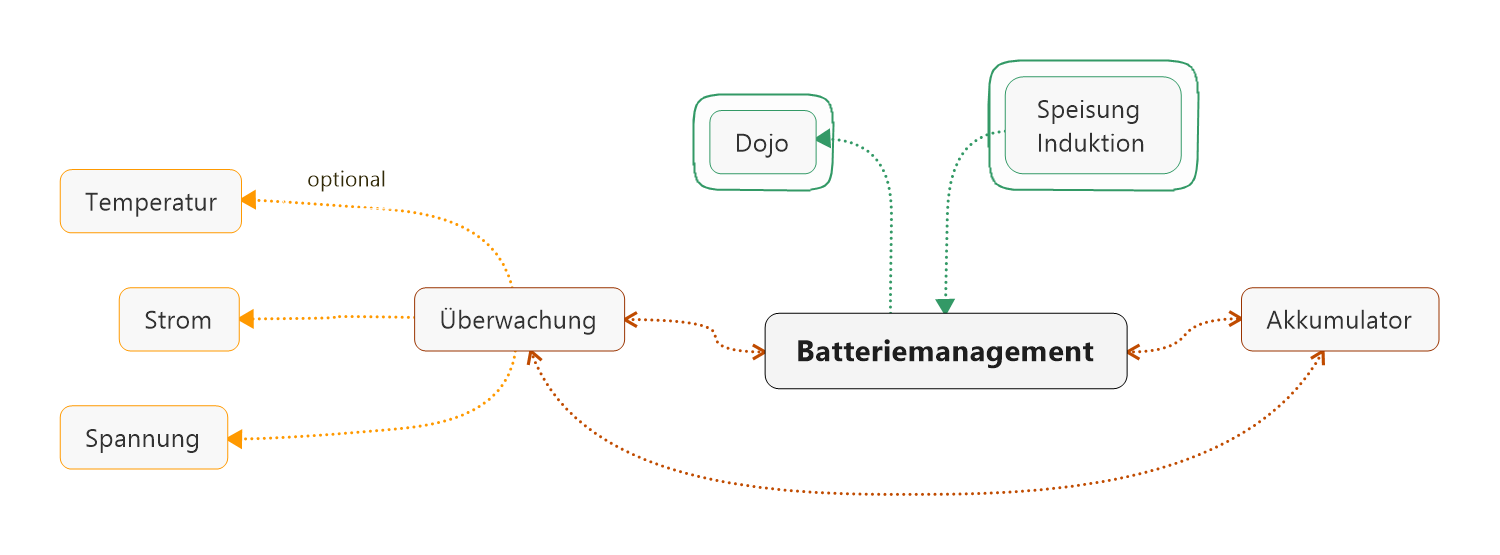
\includegraphics[width=160mm]{data/Batteriemanagement.png}
		\caption{Blockschaltbild Energiespeicherung} %picture caption
		\label{fig:blockschaltbild}
	\end{center}
\end{figure}

Das Batteriemanagement bildet den Kern der gesamten Einheit und übernimmt, wie der Name schon sagt, das gesamte Management zwischen Batterie und Speisung. Der Akkumulator wird durch Überwachungsparameter wie Strom und Spannung überwacht und übernimmt die gesamte Energieversorgung des Dojos. Die Überwachung der Temperatur ist lediglich notwendig falls eine Schnellladefunktion implementiert wird. Dieses Zusatzfeature bleibt aber als Wunschziel und wird in erster Linie nicht weiterverfolgt.

\subsection{Speicher}
Der Akkumulator besteht aus Lithium-Ionen Zellen, welche zusammen eine Spannung von 3.6V aufweisen. Aufgrund der 17mm Innendurchmesser des Dojos, sind die Abmessungen und somit auch die Auswahl an möglichen Energiespeichern relativ fix gegeben. Die notwendige Kapazität kann durch die zwei Faktoren Zeit und Energieverbrauch berechnet werden. Die Betriebszeit sollte hierbei rund 8h betragen, so dass ein Betrieb ohne Ladezyklus möglich ist. Da der Knochenschallgeber bereits eine maximale Leistung von einem Watt aufweist, liegt dementsprechend auch die maximale Leistung beim Dojo über einem Watt (nach ersten Abschätzungen bei maximal 1.2W). Nachfolgende Berechnung ergibt einen Einblick in die Kapazitätsabschätzung.

\begin{equation}
Q=\frac{t\cdot P}{U}=\frac{8h\cdot 1.2W}{3.6V}=2.67Ah
\label{fig:kapazitaet}
\end{equation}

Die geforderte Kapazität liegt gemäss Formel \ref{fig:kapazitaet} bei 2.67Ah. Unabhängig von der Grösse der Batterie ist der Schutz vor äusseren Einflüssen. Hierbei kann mittels einer gezielten Überwachung die Lebensdauer der Batterie wesentlich verlängert und die anfallenden Nebenkosten vermindert werden. Diese Thematik wird im nachfolgenden Unterkapitel \ref{Überlade und Entladeschutz} genauer erläutert.
                                         
\subsection{Überlade und Entladeschutz}  \label{Überlade und Entladeschutz}

Der Überlade- und Entladeschutz, besteht aus der Überwachung des Ladeprozesses wie auch der Signalisation bei Unterschreitung einer definierten Spannungsschwelle. Die Überwachung beim Ladezyklus erfolgt durch eine Spannungsüberwachung welche wie in Abbildung \ref{fig:Ladekurve Li-Ion Akku} ersichtlich erfolgt. Hierbei ist gut ersichtlich, dass die letzten ca. 20\% der Aufladung auf einem Spannungslevel von 4.2V erfolgen. Für die Regelung wird ein Batteriemanagement-IC vom Typ MCP73871-2CCI/ML verwendet.
Während dem Ladevorgang können hierbei zusätzlich 3 LED angesteuert werden, welche den Ladefortschritt von hoch bis tief visualisieren können. Diese drei Ladestatus zeigen den Ladefortschritt von «niedrig», «mittel» bis «gut» an. Für die Entladeüberwachung kann die Ausgabe der Ladeerkennung «niedrig» verwendet werden um das gesamt System herunterzufahren und so den Akku vor Tiefentladung zu schützen.

\begin{figure}[H]
	\begin{center}
		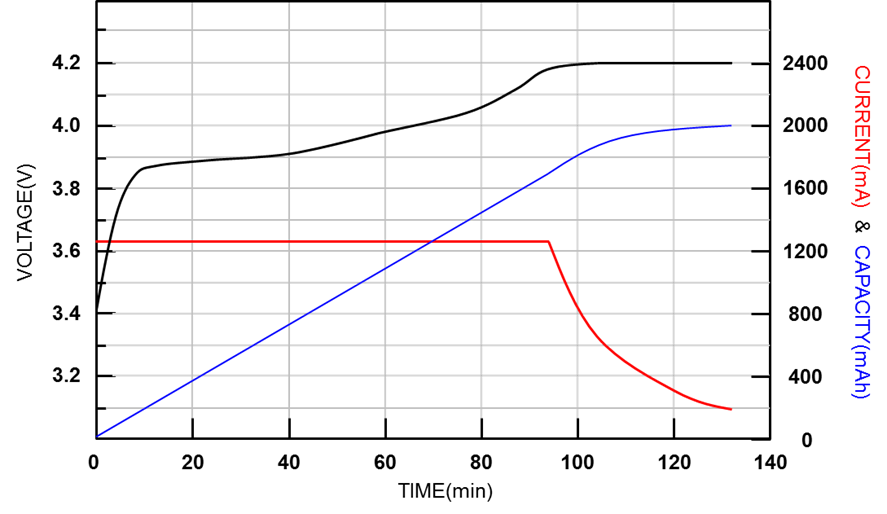
\includegraphics[width=120mm]{data/LadekurveLiIon.png}
		\caption{Blockschaltbild Energiespeicherung} %picture caption
		\label{fig:Ladekurve Li-Ion Akku}
	\end{center}
\end{figure}
